\newpage
\section{Phase d'analyse : des besoins aux fonctionnalités}
	\paragraph{}
	Intorduction de la partie.
	
	\subsection{L'enquête permet une meilleure compréhension des besoins des utilisateurs}
		\paragraph{}
		Introduction de la sous partie.
		
		\subsubsection{Élaboration d'un questionnaire d'enquête et conduite des entretiens}
			\paragraph{}% Les objectifs de l'enquêtes
			L'enquête poursuit deux objectifs :
			\begin{itemize}
			  \item D’une part nous souhaitons pouvoir établir une liste de besoins.
			  \item D’autre part, cette enquête sera l’occasion de comprendre un peu
			  mieux comment sont organisés les DSIO (direction des services informatique
			  et de l’organisation) des établissements hospitaliers, ainsi que les types
			  d’utilisateurs des consoles de supervision.
			\end{itemize}
			
			\paragraph{}% Les grands thèmes abordés
			Pour répondre à ces deux objectif, le questionnaire d’enquête doit être le
			plus générale possible. Ainsi, nous conduirons les entretiens en suivant le
			plan de questionnaire suivant :
			\begin{itemize}
			  \item[- Identification de la personne, exploration du contexte] . Cette
			  partie aura pour but de nous aider à comprendre comment est organisé le
			  service et qui est notre interlocuteur.
			  \item[- Utilisations et utilisateurs de Cloverleaf et problématique de la
			  supervision des flux] . Dans cette partie nous poserons des questions sur
			  la manière dont est utilisé Cloverleaf et par qui ainsi que les personnes
			  qui sont en charge de la supervision.
			  \item[- Attentes par rapport aux consoles de supervision] Cette partie,
			  beaucoup plus abstraite, servira à comprendre ce qu’est la supervision
			  pour les utilisateurs de consoles et quels sont les attentes des
			  utilisateurs sur les consoles de supervision.
			  \item[- Les consoles actuelles] Ces questions viseront à explorer ce que
			  les utilisateurs utilisent le plus dans les outils existant, quels sont
			  les manques et les améliorations qu’ils proposent. Cette partie explorera
			  également les propositions des utilisateurs concernant un future module
			  statistique.
			\end{itemize}
			
			\paragraph{}% Conduite des entretiens
			Les entretiens sont conduit de manière semi-directive par téléphone ou en
			face à face quand cela est possible.
			Les questions ne sont que des guides pour orienter la discussion, c’est
			pourquoi elles sont les plus ouvertes possible.\newline
			Le questionnaire a vocation à évoluer d’un entretien à un autre : des
			questions peuvent être modifiées, supprimées ou ajoutées de façon à obtenir
			des informations de plus en plus pertinentes. Chaque entretien donne lieu à
			un compte-rendu détaillé dont la structure reprend la trame du
			questionnaire. Le questionnaire, dans sa version finale, se trouve en annexe
			A.
			
			\paragraph{}% Les principes de l'étude qualitative
			Il s'agit d'une étude qualitative. Contrairement aux études quantitatives qui
			permettent de récolter des données repérsentatives d'une population,
			dans une étude qualitative nous ne cherchons pas à interroger le plus de
			monde possible. Les entretients sont basés sur des question ouverte et durent
			en général plus longtemp que dans des enquêtes quantitatives. L'objetcif
			d'une telle étude est de faire ressortir la diversité des comportement. Dans
			notre cas, il s'agit de mettre en avant les différentes utilisations
			possibles des consoles de supervision et ses utilisateurs.
			
			\paragraph{}% Choix de la population interrogée
			Un panel de 5 établissements hospitaliers est interrogé. Tous ces
			établissements sont des clients d’Xperis :
			\begin{itemize}
			  \item Tour
			  \item Toulouse
			  \item Rouen
			  \item Brest
			  \item Metz
			\end{itemize}
			
			\paragraph{}% Méthodes d'analyse des résultat
			A l'issue des enquêtes nous procéderons à l'analyse des résultats. Après une
			rapide relecture de tous les comptes rendu d'entretien, nous établissons une
			listes des grands thèmes qui ont été abordés durant les discussion. Nous
			classons ensuites toutes les informations collectées dans ces thèmes.\newline
			Les thèmes qui sont ressortis sont les suivants :
			\begin{itemize}
			  \item[- grand thème 1] L’organisation des services informatique dans les
			  hôpitaux,
			  \item[- grand thème 2] Les types d’utilisateurs de TC,
			  \item[- grand thème 3] Les types d’utilisations de TC,
			  \item[- grand thème 4] Les attentes par rapport aux consoles de supervision
			  et la réponse des outils actuels à ces attentes,
			  \item[- grand thème 5] Les fonctionnalités manquant aux consoles de
			  supervisions actuelles,
			  \item[- grand thème 6] Les statistiques sur les flux.
			\end{itemize}
			Dans la suite de cette partie nous entrerons dans le détail des informations
			collectées pour chacun de ces grand thèmes.
			
		\subsubsection{La supervision fait partie du processus de résolution des
		anomalies}
			\paragraph{}% Présentation
			Nous analyserons ici l'organisation interne des services liées à
			l'interopérabilité dans les hôpitaux. Nous verons ensuite quelles sont les
			pratiques liées à la supervision (autrement dit, nous détaillerons les
			grands thèmes 1 et 3).
			
			\paragraph{}% L'organisation des DSIO
			Les services informatiques ont des structures variables selon les
			établissements. Cependant, il existe dans tous les cas observés au moins un
			département consacré à l’interopérabilité. Ce département peut se subdiviser
			en deux pôles :
			\begin{itemize}
			  \item Un pôle intégration
			  \item Un pôle exploitation
			\end{itemize}
			Le pôle intégration prend en charge la mise en place de nouveaux flux et du
			bon fonctionnement de l’EAI. Son niveau de compétence sur Cloverleaf est
			élevé. Ce type de pôle existe dans des établissements relativement autonomes
			vis-à-vis des éditeurs. Le pôle intégration se compose généralement de 2 à 3
			personnes. Les outils utilisés sont principalement l’IDE, EAI Supervision et
			Global Monitor (GM).\\
			Le pôle exploitation a en charge la supervision des flux. Le niveau de
			maîtrise de Cloverleaf y est plus faible. Les outils utilisés sont en
			général les consoles de supervision (GM, TC, EAI supervision), mais pas
			l’IDE, trop complexe pour ce type d’utilisateur.\\
			Les deux pôles peuvent cohabiter au sein d’un même établissement. Certains,
			comme le CHU de Metz, n’ont qu’un pôle exploitation, la mise en place des
			flux étant assuré par un autre département (en l’occurrence, le département
			en charge de l’urbanisation). D’autres établissements, beaucoup plus
			dépendants des éditeurs, ne s’occupent pas de la mise en place des flux ni
			du fonctionnement de l’EAI, mais seulement de la supervision. C’est par
			exemple le cas du CHU de Châtellerault.\\
			La Figure 5 résume les différents niveaux de gestion de l’interopérabilité au
			sein d’un hôpital. Un pôle exploitation se situe au niveau le plus bas
			tandis qu’un pôle intégration peut se situer au niveau 2 ou 3. Le niveau le
			plus haut est en général assuré par un département urbanisation, en charge
			de la définition de la politique de tout le SI.
			% Niveau de responsabilité pour l'interop dans le SI
			\begin{figure}[!h]
				\centering
				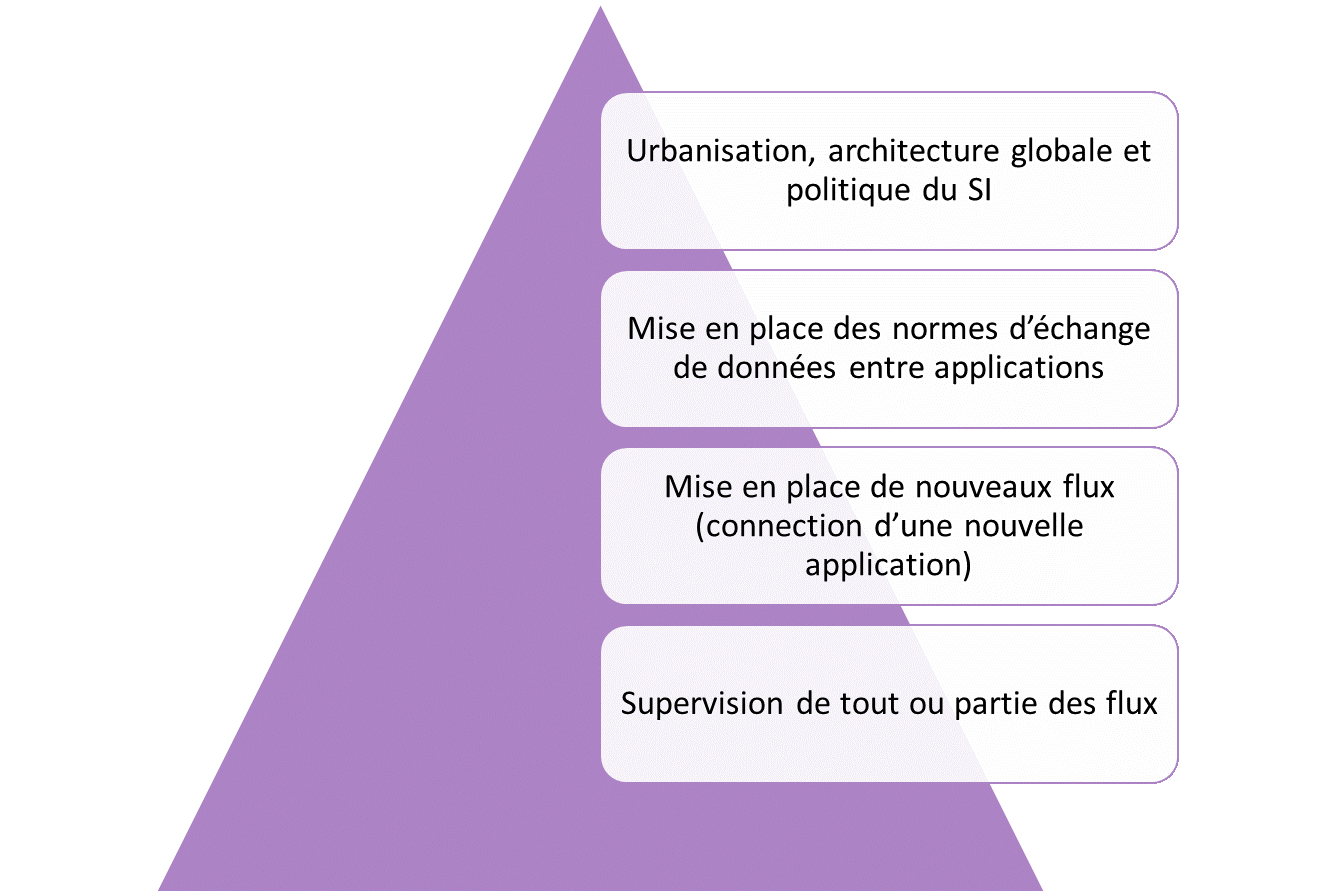
\includegraphics[width=8cm]{../img/si_1.png}
				\caption{\label{Figure 4} Les différents niveaux de responsabilité autour
				de la gestion de l'interopérabilité.}
			\end{figure}
			
			\paragraph{}% Diversité des pratiques
			L’ensemble des outils liés à Cloverleaf (IDE et consoles de supervision) sont
			utilisés pour la supervision des flux. Les utilisateurs les plus aguerris
			sur Cloverleaf utilisent l’IDE, notamment le bouton status qui donnes accès
			à des données statistiques sur un thread ou un process. Pour détecter les
			problèmes, l’utilisateur se fie principalement à l’heure de dernière
			écriture d’un message. Si rien n’a été écrit depuis un certain temps, c’est
			que le flux est bloqué et que les messages ne passent plus. Ce type
			d’utilisateur est généralement en charge de la résolution des problèmes les
			plus complexes. Pour cela, il a parfois recours à la consultation de l’error
			database ou des SMAT pour comprendre l’origine de l’erreur.\\
			Du côté des consoles de supervision, les usages qui sont ressortis sont :
			\begin{itemize}
			  \item Visualiser l’état des flux (si les threads et process sont bien en
			  marche),
			  \item Affichage sur écran géant,
			  \item Rechercher un message en particulier, ou un certain type de
			  messages. Par exemple, tous les messages concernant un patient donné,
			  \item Visualiser les messages en erreur,
			  \item Supervision en mode lecture seule : vérifier que les messages
			  passent bien et connaître l’origine des erreurs,
			  \item Explorer le contenu des messages pour diagnostiquer une erreur,
			  \item Réaliser des tests lors de la mise en place de flux (usage repéré
			  uniquement au CHU de Toulouse),
			  \item Editer le contenu des messages en cas d’erreur,
			  \item Rejouer des messages après les avoir édités,
			  \item Pour les flux Maincare et EAI Supervision, s’assurer que les
			  messages sont bien intégrés dans les applications de destination,
			  \item Restreindre l’utilisation de certaines fonctionnalités pour par
			  exemple confier les outils à des personnes d’astreintes ou des personnes
			  métier,
			  \item Comparer le contenu d’un message entre son entrée dans un flux et
			  sa sortie. Cet usage n’a été référencé que pour EAI Supervision,
			  \item Paramétrer l’outil : création de colonnes, attribution des droits…
			\end{itemize}
			\paragraph{}
			Cette liste nous permet de connaître les principales utilisations des
			consoles de supervision \ref{Figure x}. L’utilisation la plus simple est la
			visualisation : voir les messages qui passent et pouvoir détecter rapidement
			les erreurs. Une fois les erreurs détectées, l’utilisateur cherche à
			comprendre ce qui les a causées. Pour cela, il peut être suffisant de
			regarder le contenu du message pour en repérer les anomalies, ou bien aller
			dans l’error database. Une fois la cause de l’erreur bien établie, vient une
			phase de correction. Celle-ci peut se faire par édition du contenu du
			message et par rejoue, dans les cas les plus simples. Comme c’est le cas
			pour le CHU de Toulouse, la console peut être utilisée pour effectuer des
			tests lors de la mise en place de nouveaux flux. C’est-à-dire vérifier que
			les messages passent correctement d’une application à une autre. Enfin, les
			utilisateurs les plus avertis ont en charge l’administration de la console,
			c’est-à-dire son paramétrage (attribution des droits de consultation et
			d’action aux utilisateurs, paramétrage des colonnes …). Ce rôle revient
			généralement au pôle intégration ou à Xperis. On remarque que, dans le cas
			de TC, le paramétrage de la console est un facteur limitant à son
			utilisation en production.
			% Niveau de responsabilité pour l'interop dans le SI
			\begin{figure}[!h]
				\centering
				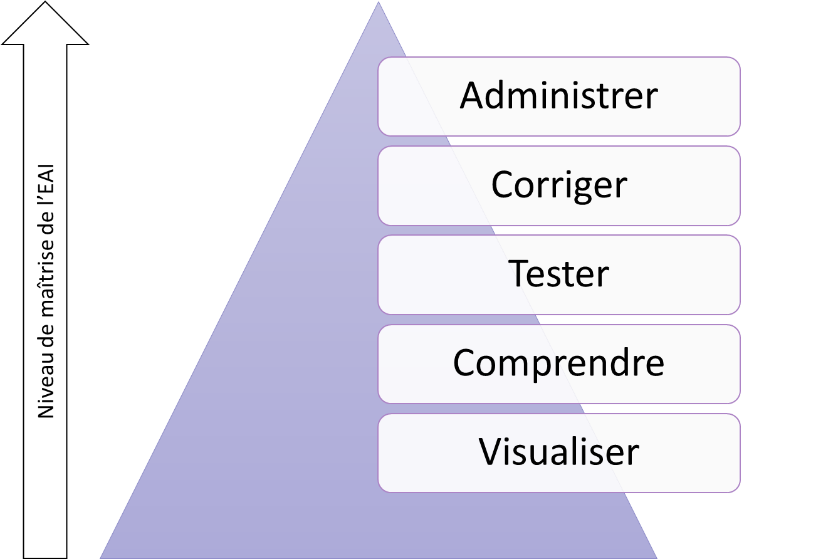
\includegraphics[width=8cm]{../img/usage_1.png}
				\caption{\label{Figure x} Les différents d'utilisation des consoles de
				supervision.}
			\end{figure}
			
			\paragraph{}
			En bilan, nous pouvons définir la supervision d'un flux comme :
			\begin{itemize}
			  \item Voire en un coup d’œil la présence d’anomalies telles que :
			  	\begin{itemize}
			  	  \item Des erreurs,
			  	  \item Des ralentissements,
			  	  \item Des blocages
		  	    \end{itemize}
			  \item Pouvoir expliquer, même partiellement ces anomalies,
			  \item Et éventuellement pouvoir agir dessus, par exemple en rejouant un
			  message qui n’est pas passé à cause d’un problème momentané de la connexion.
			\end{itemize}
			
		\subsubsection{Une grande diversité des utilisateurs des consoles de
		supervision}
			\paragraph{}% Présentation
			Nous présenterons ici la typologie d'utilisateur qui est ressortie de
			l'étude, ce qui correspond au grand thème 2.
			
			\paragraph{}% Les utilisateurs
			
		\subsubsection{L'enquête permet de dresser une liste des besoins}
			\paragraph{}% La notion de besoin
			
			\paragraph{}% Les attentes qui sont ressorties de l'enquête
			
			\paragraph{}% La lise des besoins
			A partir des entretiens, nous avons dresser une liste de besoins de natures
			diverse. Ceux-ci consernent différents aspect de TrackCIS ou de la
			supervision. On peut les classer dans différentes catégories :
			\begin{itemize}
			  \item Les besoins
			\end{itemize}
	
	\subsection{La liste des besoins permet de dresser une liste de fonctionnalités}
		\paragraph{}% On ne se concentre que sur les besoins liés aux stats
		Nous avons dressé et analysé une liste de besoins émanant d'utilisateur
		concernant la supervision. Notre projet ne vise pas à traiter l'intégralité de
		ces besoins. Nous ne nous focaliserons ici que sur les besoins relatifs à un
		module de consultation de statistiques.
		
		\subsubsection{De la liste des besoins à la liste des fonctionnalités}
			\paragraph{}% Mode de passage des besoins aux fonctionnalités
			
			\paragraph{}% Formalisation des fonctionnalités grace au diagramme FODA
			
		\subsubsection{Priorisation des fonctionnalités liées aux statistiques}
			\paragraph{}% But de la priorisation des fonctionnalités
			
			\paragraph{}% Quelques rappels en UML
			
			\paragraph{}% Représentation des fonctionnalités liées aux stats en UML
	
	\subsection{Des fonctionnalités vers les cas d'utilisation}
		\paragraph{}
		Introduction de la sous partie.
		
		\subsubsection{État de l'art sur les consoles de supervision et la visualisation de données}
			\paragraph{}
			Texte de la sous sous partie
		\subsubsection{Choix des modes de visualisation par le biais de maquettes}
			\paragraph{}
			Texte de la sous sous partie
		\subsubsection{Création de scénarios d'utilisation}
			\paragraph{}
			Texte de la sous sous partie
